\subsection{Effective Lagrangian Description as a Hydrodynamic Limit}
  \label{subsec:effective-lagrangian-description}
  \textit{Note on the status of the effective action: The comprehensive Lagrangian density presented in this appendix
is not to be interpreted as a fundamental axiomatic starting point.
In the Cosmochrony framework, the fundamental dynamics resides in the irreversible relaxation of the $\chi$ field on a
discrete relational network (see Appendix~\ref{subsec:relational_foundation}).
The standard Einstein-Dirac-Maxwell action is presented here as a \textbf{reconstruction a posteriori}.
It serves as a proof of concept to demonstrate how the emergent degrees of freedom—specifically localized solitonic
excitations—map onto the effective field theories of the Standard Model and General Relativity.}

\paragraph{From Discrete Network to Continuum.}
  As established in the relational foundation, the collective behavior of the graph $G(V,E)$ can be mapped onto a
  continuous effective action. In this framework, the connectivity $K_{uv}$ between nodes is not a static background
  but a \textbf{dynamic measure} of the local $\chi$-field gradient, representing the relational tension between units:
  \begin{equation}
    K_{uv} \propto \frac{1}{1 - \frac{(\Delta \chi_{uv})^2}{c^2 \Delta \ell^2}}
  \end{equation}
  where $\Delta \chi_{uv}$ is the field variation between adjacent nodes, and $\Delta \ell$ denotes a fixed
  combinatorial link scale of the graph---not a physical spatial distance.
  The operational distance $d(i,j)$ is then defined as the geodesic distance on this weighted graph:
  \begin{equation}
    d(i,j) = \min_{p \in \mathcal{P}_{ij}} \sum_{(u,v) \in p} \frac{1}{\sqrt{K_{uv}}}
  \end{equation}
  where $\mathcal{P}_{ij}$ is the set of all paths connecting $i$ and $j$, and the $\sqrt{K_{uv}}$ dependence
  reflects the Born--Infeld–type non-linearity of the $\chi$-field dynamics and ensures
  that the emergent metric respects the fundamental gradient bound set by $c$.
  This definition ensures that the geometry is a secondary consequence of the field's local state.

\paragraph{Local Metric Reconstruction.}
  The metric tensor $g_{\mu\nu}(x)$ is an effective local field reconstructed from this connectivity.
  For any small displacement $\Delta x^\mu$ in the continuum, the components $g_{\mu\nu}$ are determined such that the
  quadratic form matches the infinitesimal operational distance of the network:
  \begin{equation}
    g_{\mu\nu}(x) \Delta x^\mu \Delta x^\nu \approx \delta \ell^2_{network}
  \end{equation}
  Spatial inhomogeneities in the connectivity density $K_{uv}$ modify the geodesic structure of the underlying network.
  In this view, the curvature of spacetime (gravity) is the macroscopic manifestation of these connectivity gradients,
  induced by localized $\chi$-field configurations (matter).

\subsubsection{Gravity and Time: The Geometric Relaxation Term ($\mathcal{L}_{\text{Gravity/Time}}$)}
This term ensures the emergence of GR and imposes the arrow of time. In the continuous limit:
\begin{equation}
  \mathcal{L}_{\text{Gravity/Time}} = \frac{1}{16\pi G_{\text{eff}}} R + \lambda (\partial_t \chi - c \sqrt{1 - |\nabla \chi|^2/c^2})
\end{equation}
The second term acts as a constraint in the effective theory, enforcing the unit-velocity relaxation derived from the
fundamental network dynamics.

\subsubsection{Field Dynamics: The Non-linear Regularizer ($\mathcal{L}_{\chi/\text{Soliton}}$)}
To prevent singular configurations at the center of solitons, the kinetic term adopts a Born-Infeld structure as
proposed in Section~\ref{subsec:variational-formulation}:
\begin{equation}
  \mathcal{L}_{\chi/\text{Soliton}} = -c^2 \sqrt{1 - \frac{|\nabla \chi|^2}{c^2}} - V_{\text{Soliton}}(\chi)
\end{equation}
This ensures that the gradient magnitude $|\nabla \chi|$ is bounded by $c$, naturally regularizing the self-energy of
solitons (particles).

\subsubsection{Emergent Forces and Matter ($\mathcal{L}_{\text{Forces/Matter}}$)}

This encompasses the emergent field theories: electromagnetism (photons, $A_\mu$) and fermionic matter (electrons,
$\Psi$) which are understood as dynamic excitations of the $\chi$-field.

\[\mathcal{L}_{\text{Forces/Matter}} = - \frac{1}{4} F_{\mu\nu} F^{\mu\nu} + \mathcal{L}_{\text{Dirac}}^
  {\text{Torsion}}(\chi, \Psi)\]

\begin{itemize}
  \item $F_{\mu\nu}$ is the electromagnetic field strength tensor, whose dynamics emerge as low-frequency $\chi$
  -fluctuations.
  \item $\mathcal{L}_{\text{Dirac}}^{\text{Torsion}}$ is the emergent Lagrangian for fermionic matter fields $\Psi$. Crucially, it must be formulated in an **affine manifold with Torsion $T$** (where $T$
  is geometrically induced by the $\chi$-field dynamics). The Torsion term is vital as it provides the geometric interpretation of the spin $1/2$
  constraint and the Pauli Exclusion Principle.
  \item The mass term for the emergent Dirac field is $m_{\text{eff}}(\chi)$, reflecting the energy required to sustain the local $\chi$-soliton configuration.
\end{itemize}

\medskip
This full Lagragian provides the formal starting point for the field equations, the quantitative resolution of
which is required to rigorously demonstrate the structural emergence of all standard physical laws.

\subsubsection{On the Microscopic Origin of the Coupling $S[\chi, \rho]$}
While the source term $S[\chi, \rho]$ is presented phenomenologically in the effective theory to recover the Poisson
equation, its origin in Cosmochrony is strictly relational.

In the discrete network $G(V,E)$, matter (solitons) corresponds to regions where the field gradient $\Delta \chi$ is
maximal.
According to the dynamic connectivity rule:
\begin{equation}
  K_{ij} = f(\Delta \chi_{ij})
\end{equation}
the presence of a soliton locally alters the connectivity density. Since the relaxation rate $\partial_t \chi$ depends
on the Laplacian $\sum K_{ij} \Delta \chi_{ij}$, any modification of $K_{ij}$ by a matter configuration acts as a local
impedance to the global relaxation flow.

Therefore, $S[\chi, \rho]$ is not an independent coupling constant but the continuum limit of the
\textbf{structural feedback} of the network's topology on its own dynamics.
The linearity of $S \propto \rho$ in the weak-field limit is an emergent property of this feedback at large scales.


\subsection{Nature of the $\chi$ Field}
  \label{subsec:nature-of-the-$chi$-field}
  The field $\chi(x^\mu)$ is postulated as a real scalar field defined on a four-dimensional differentiable manifold.
Unlike conventional scalar fields in quantum field theory, $\chi$ does not represent a matter degree of freedom propagating
\emph{within} spacetime.
Instead, it encodes the local geometric scale governing the emergence of spacetime itself.

Operationally, $\chi$ may be interpreted as a proper wavelength field whose monotonic increase defines both spatial
separation and temporal flow.


\subsection{Stability Analysis of the $\chi$-Field Dynamics}
  \label{subsec:stability_chi}
  The stability of the $\chi$-field dynamics, governed by $\partial_t \chi = c \sqrt{1 - |\nabla \chi|^2/c^2}$,
describes the irreversible relaxation of $\chi$, where $c$ is the maximal relaxation speed.

It is essential to ensure that Cosmochrony provides a \textbf{physically consistent and predictive framework}.
Without stability, small perturbations could lead to unphysical divergences, compromising the theory's
ability to unify gravity, quantum mechanics, and cosmology.
This analysis confirms that the $\chi$ field remains well-behaved under perturbations,
validating its role as a fundamental geometric substrate for spacetime and matter.

Below, we demonstrate its stability under small perturbations, both in linear and nonlinear regimes.

\subsubsection{Linear Stability}

  Consider a spatially homogeneous base state, $\chi_0(t) = ct + \chi_{0,0}$, satisfying $\partial_t \chi_0 = c$
  . Let $\chi(x,t) = \chi_0(t) + \delta \chi(x,t)$, where $|\delta \chi| \ll |\chi_0|$
  . Substituting into the governing equation and linearizing yields:

  \[
    \partial_t \delta \chi = -\frac{|\nabla \delta \chi|^2}{2c}.
  \]

  Since the right-hand side is non-positive, \textbf{small perturbations decay over time}
  , ensuring linear stability.

\subsubsection{Nonlinear Stability}

  To assess nonlinear stability, we introduce an energy-like functional:

  \[
    E[\delta \chi] = \frac{1}{2} \int |\nabla \delta \chi|^2 \, d^3x.
  \]

  The time derivative of $E$ is:

  \[
    \frac{dE}{dt} = \int \nabla \delta \chi \cdot \nabla (\partial_t \delta \chi) \, d^3x.
  \]

  Substituting the linearized equation, we find that $E$
  is non-increasing, confirming that perturbations remain bounded. A Lyapunov functional can also be
  constructed to show that the system is \textbf{nonlinearly stable}.

\subsubsection{Special Cases}

  \begin{itemize}
    \item \textbf{Planar Waves:} For $\delta \chi = \epsilon \sin(kx - \omega t)$, the dispersion relation
    $\omega = \frac{c k^2}{2 \chi_0}$ shows that high-wavenumber perturbations are strongly damped.
    \item \textbf{Spherical Symmetry:} For $\delta \chi(r,t)$
    , the linearized equation admits diffusively decaying solutions.
  \end{itemize}

\subsubsection{Conclusion}

  The $\chi$-field dynamics are \textbf{stable}
  under both linear and nonlinear perturbations. This stability supports the viability of $\chi$
  as a fundamental field underlying spacetime, gravity, and quantum phenomena in Cosmochrony.


\subsection{Analytical Solutions of the \(\chi\)-Field Dynamics}
\label{sec:analytical_solutions_chi}

To illustrate the behavior of the \(\chi\)
field, we derive explicit analytical solutions of the dynamical equation
\[
  \partial_t \chi = c \sqrt{1 - \frac{|\nabla \chi|^2}{c^2}},
\]
in two simple but physically relevant cases: \textbf{homogeneous configurations} and
\textbf{spherically symmetric solutions}.

\subsubsection{Homogeneous Solution}
  In a spatially homogeneous universe, \(\nabla \chi = 0\). The dynamical equation reduces to:
  \[
    \partial_t \chi = c.
  \]
  Integrating with respect to time, we obtain the trivial but fundamental solution:
  \[
    \chi(t) = \chi_0 + c t,
  \]
  where \(\chi_0\) is the initial value of \(\chi\). This solution describes the
  \textbf{background cosmological expansion} in Cosmochrony, where \(\chi\)
  grows linearly with time, directly yielding a Hubble-like law for the scale factor \(a(t) \propto \chi(t)\).

\subsubsection{Spherically Symmetric Solution}
  Consider a spherically symmetric configuration, where \(\chi = \chi(r,t)\) and the gradient reduces to
  \(\nabla \chi = \partial_r \chi \, \hat{r}\). The dynamical equation becomes:
  \[
    \partial_t \chi = c \sqrt{1 - \frac{(\partial_r \chi)^2}{c^2}}.
  \]

  To find a stationary solution (\(\partial_t \chi = 0\)), we set:
  \[
    c \sqrt{1 - \frac{(\partial_r \chi)^2}{c^2}} = 0 \implies \partial_r \chi = \pm c.
  \]

  Integrating, we obtain:
  \[
    \chi(r) = \chi_0 \pm c r,
  \]
  where \(\chi_0\) is an integration constant. This solution represents a \textbf{conical profile} for \(\chi\)
  , with a gradient maximal (\(|\nabla \chi| = c\)
  ). While this solution is not physically realizable globally (as it violates the boundedness of \(\chi\)
  ), it illustrates the extreme case where the relaxation of \(\chi\)
  is maximally slowed by spatial gradients.

  For a more realistic, time-dependent solution, assume a separable ansatz \(\chi(r,t) = R(r)T(t)\)
  . Substituting into the dynamical equation and separating variables, we find:
  \[
    \frac{\dot{T}}{c \sqrt{1 - \frac{T^2 (R')^2}{c^2}}} = 1.
  \]
  This implies \(\dot{T} = c\), so \(T(t) = c t + T_0\). The spatial part \(R(r)\) must then satisfy:
  \[
    (R')^2 = \frac{c^2}{T^2} \left(1 - \frac{1}{c^2}\right).
  \]
  For \(T(t) = c t\), this simplifies to:
  \[
    R(r) = R_0 \pm r,
  \]
  yielding the time-dependent solution:
  \[
    \chi(r,t) = \chi_0 + c t \pm r.
  \]
  This solution describes a \textbf{propagating front} of \(\chi\), where the field grows linearly with time and varies linearly with radius.
  It is particularly relevant for modeling localized excitations, such as particle-like solitons, in a spherically symmetric geometry.

\subsubsection{Planar Wave Solution}
  For a planar wave ansatz \(\chi(x,t) = \chi_0 + \delta \chi(x,t)\), where \(\delta \chi\)
  represents a small perturbation, we linearize the dynamical equation:
  \[
    \partial_t \delta \chi = -\frac{(\partial_x \delta \chi)^2}{2c}.
  \]
  Assuming a wave-like perturbation \(\delta \chi = \epsilon \sin(kx - \omega t)\),
  we substitute into the linearized equation and find the dispersion relation:
  \[
    \omega = \frac{c k^2}{2 \chi_0}.
  \]
  This shows that \textbf{high-wavenumber perturbations are strongly damped},
  confirming the stability of the homogeneous solution against small-scale fluctuations.
  The planar wave solution is particularly useful for modeling propagating disturbances in \(\chi\),
  such as gravitational waves or electromagnetic radiation in the Cosmochrony framework.

\subsubsection{Conclusion}
  These analytical solutions illustrate the rich dynamical behavior of the \(\chi\)
  field in simple but physically meaningful configurations.
  The homogeneous solution underpins the cosmological expansion,
  while the spherically symmetric and planar wave solutions provide insights into localized excitations and propagating disturbances.
  Together, they confirm the consistency and versatility
  of the \(\chi\)-field dynamics as a unifying framework for spacetime, gravity, and quantum phenomena.

\subsection{Coupling with Matter: The \(S[\chi, \rho]\) Term in the Effective Wave Equation}
\label{sec:coupling_matter_chi}

The effective wave equation for the \(\chi\) field in Cosmochrony includes a source term \(S[\chi, \rho]\)
that captures the interaction between \(\chi\) and matter (or energy) density \(\rho\):
\[
  \square \chi = S[\chi, \rho].
\]
This term is \textbf{critical}
for understanding how localized excitations (e.g., particles, black holes) influence the relaxation of
\(\chi\), leading to emergent phenomena such as gravity, time dilation, and quantum localization.
Below, we discuss its functional form, physical interpretation, and implications for the robustness of the model.

\subsubsection{Physical Interpretation of \(S[\chi, \rho]\)}
  The term \(S[\chi, \rho]\) represents the
  \textbf{resistance of matter excitations to the relaxation of \(\chi\)}.
  Physically, it encodes how the presence of matter or energy density \(\rho\) modifies the local dynamics of \(\chi\),
  slowing its evolution and inducing spatial gradients.
  This mechanism underlies several key predictions of Cosmochrony:

  \begin{itemize}
    \item \textbf{Gravitational time dilation}: Regions with higher \(\rho\) exhibit slower \(\chi\)
    relaxation, leading to time dilation effects analogous to those in general relativity.
    \item \textbf{Particle mass}: Localized excitations (solitons) correspond to stable configurations of \(\chi\)
    where \(S[\chi, \rho]\) balances the relaxation tendency, giving rise to inertial mass.
    \item \textbf{Curvature of spacetime}: Spatial variations in \(\chi\) relaxation, driven by \(S[\chi, \rho]\), induce an effective metric structure that reproduces gravitational phenomena.
  \end{itemize}

\subsubsection{Functional Form of \(S[\chi, \rho]\)}
  The exact form of \(S[\chi, \rho]\)
  is not yet fully determined from first principles, but we can infer its general properties based on physical
  requirements:

  \begin{enumerate}
    \item \textbf{Linearity in \(\rho\) (Weak-Field Limit)}:
    In regimes where \(\rho\) is small (e.g., weak gravitational fields), \(S[\chi, \rho]\)
    is expected to be linear in \(\rho\):
    \[
      S[\chi, \rho] \approx -\alpha \rho,
    \]
    where \(\alpha\)
    is a coupling constant. This form reproduces Newtonian gravity in the weak-field limit, where the
    gravitational potential \(\Phi\) satisfies \(\nabla^2 \Phi \propto \rho\). Comparing with general relativity, we identify \(\alpha \sim G/c^2\), where \(G\)
    is Newton's gravitational constant.

    \item \textbf{Nonlinear Dependence (Strong-Field Regime)}:
    For high matter densities (e.g., near black holes or in the early universe), \(S[\chi, \rho]\)
    may include nonlinear terms to prevent unphysical divergences:
    \[
      S[\chi, \rho] = -\alpha \rho
      \left(1 + \beta \frac{\rho}{\rho_c} + \gamma \frac{\rho^2}{\rho_c^2} + \cdots \right),
    \]
    where \(\rho_c\) is a critical density scale (e.g., Planck density), and \(\beta, \gamma\)
    are dimensionless coefficients. Nonlinearities ensure that \(\chi\) relaxation does not halt completely (
    \(\partial_t \chi \geq 0\)) even in extreme regimes.

    \item \textbf{Dependence on \(\chi\)}:
    The coupling may also depend on \(\chi\)
    itself, reflecting the self-interaction of the field. A plausible ansatz is:
    \[
      S[\chi, \rho] = -\alpha(\chi) \rho,
    \]
    where \(\alpha(\chi)\) could take the form \(\alpha(\chi) = \alpha_0 (1 - \chi/\chi_{\max})\)
    to enforce the boundedness of \(\chi\). This ensures that the relaxation rate \(\partial_t \chi\)
    remains positive and physically meaningful.
  \end{enumerate}

\subsubsection{Implications for Gravitational Phenomena}
  The form of \(S[\chi, \rho]\) directly impacts the emergent gravitational dynamics in Cosmochrony:

  \begin{itemize}
    \item \textbf{Newtonian Limit}: For weak fields, the linear coupling \(S \approx -\alpha \rho\)
    yields the Poisson equation for the gravitational potential:
    \[
      \nabla^2 \Phi = 4 \pi G \rho,
    \]
    where \(\Phi\) is identified with deviations in \(\chi\) relaxation.

    \item \textbf{Schwarzschild Metric Recovery}: In spherically symmetric configurations, the effective metric derived from \(\chi\)
    dynamics reproduces the Schwarzschild solution when \(S[\chi, \rho]\) is linear in \(\rho\). This provides a geometric interpretation of black holes as regions where \(\chi\)
    relaxation is strongly suppressed.

    \item \textbf{Modified Gravity in Dense Regimes}: Nonlinear terms in \(S[\chi, \rho]\)
    could lead to deviations from general relativity in strong gravitational fields, offering potential signatures
    for testing Cosmochrony against observations (e.g., gravitational wave echoes, black hole shadows).
  \end{itemize}

\subsubsection{Open Questions and Future Directions}
  While the linear form of \(S[\chi, \rho]\)
  is sufficient to recover many classical gravitational effects, several questions remain open:

  \begin{itemize}
    \item \textbf{Microscopic Origin of \(\alpha\)}: What determines the coupling constant \(\alpha\)? Is it fundamental, or does it emerge from the underlying \(\chi\) dynamics?
    \item \textbf{Quantum Coupling}: How does \(S[\chi, \rho]\) behave in quantum regimes, where \(\rho\)
    corresponds to probability densities or wavefunction amplitudes?
    \item \textbf{Cosmological Implications}: Could nonlinearities in \(S[\chi, \rho]\)
    explain dark matter effects or modifications to the Hubble law at large scales?
  \end{itemize}

  Addressing these questions will require a combination of analytical work, numerical simulations, and comparisons
  with observational data.

\subsubsection{Conclusion}
  The term \(S[\chi, \rho]\) is a cornerstone of the Cosmochrony framework, linking the \(\chi\)
  field to observable
  physical phenomena. Its functional form---likely linear in weak fields but potentially nonlinear in extreme
  regimes---determines the theory's predictive power and robustness. Further exploration of \(S[\chi, \rho]\)
  will
  deepen our understanding of how matter, gravity, and spacetime emerge from the dynamics of \(\chi\).

\subsection{Topological Configurations of the \(\chi\) Field: Solitons as Particles}
\label{sec:topological_solitons}

In Cosmochrony, particles are interpreted as \textbf{topologically stable solitons} of the \(\chi\) field, where
their properties---such as \textbf{spin, charge, and mass}---emerge from the
\textbf{local deformation of \(\chi\)} and
its topological structure. Below, we classify these configurations and explicitly link them to particle properties
, emphasizing how \textbf{charge arises from the modulation of \(\chi\)'s relaxation}.

\subsubsection{Charge as Local Deformation of \(\chi\)}
  The \textbf{sign of a particle's charge} (positive or negative) is determined by how it deforms the \(\chi\)
  field:
  \begin{itemize}
    \item A \textbf{positive charge} corresponds to a \textbf{local extension of \(\chi\)} (a "peak"), which resists relaxation and repels other positive charges (as two peaks cannot merge).
    \item A \textbf{negative charge} corresponds to a \textbf{local contraction of \(\chi\)} (a "trough"), which attracts positive charges (as a peak and trough can annihilate or merge).
  \end{itemize}
  This geometric interpretation explains \textbf{Coulomb-like interactions}
  without invoking a fundamental electromagnetic field, but as a consequence of \(\chi\) dynamics.

\subsubsection{Vortices (Charged Particles with Spin)}
  Vortices in the \(\chi\) field are characterized by a quantized winding number \(n\):
  \[
    n = \frac{1}{2\pi} \oint \nabla \arg(\chi) \cdot d\mathbf{l}.
  \]
  The \textbf{charge of the vortex} is determined by the \textbf{sign of its deformation}:
  \begin{itemize}
    \item For \(n > 0\), the vortex creates a \textbf{local extension of \(\chi\)} (positive charge).
    \item For \(n < 0\), the vortex creates a \textbf{local contraction of \(\chi\)} (negative charge).
  \end{itemize}
  The energy of the vortex scales with \(n^2\), reflecting the \textbf{mass of the particle}
  , while its winding determines the \textbf{spin} (e.g., \(n=1\) for spin-1 bosons).

\subsubsection{Skyrmions (Fermions with Charge and Spin-1/2)}
  Skyrmions are 3D solitons with a topological charge \(Q\):
  \[
    Q = \frac{1}{4\pi} \int \mathbf{n} \cdot (\partial_x \mathbf{n} \times \partial_y \mathbf{n}) \, dx \, dy,
  \]
  where \(\mathbf{n} = \chi / |\chi|\). The \textbf{charge of the skyrmion} is linked to the
  \textbf{polarity of its \(\chi\) deformation}:
  \begin{itemize}
    \item A skyrmion with \(Q = +1\) and a \textbf{peak in \(\chi\)} represents a
    \textbf{positively charged fermion} (e.g., proton).
    \item A skyrmion with \(Q = -1\) and a \textbf{trough in \(\chi\)} represents a
    \textbf{negatively charged fermion} (e.g., electron).
  \end{itemize}
  The \(4\pi\)-periodicity of skyrmions under rotations explains their \textbf{spin-1/2}
  nature, while the deformation of \(\chi\) accounts for their charge.

\subsubsection{Summary: Topology and Charge}
  The relationship between topology and charge in Cosmochrony is summarized in ~\ref{tab:solitons_charge}

  \begin{table}[htbp]
    \centering
    \caption{Topological Solitons, Charge, and \(\chi\) Deformation}
    \label{tab:solitons_charge}
    \begin{tabular}{|c|c|c|c|}
      \hline
      \textbf{Soliton Type} & \textbf{Topological Invariant} & \textbf{\(\chi\) Deformation} &
      \textbf{Particle Property} \\
      \hline
      Vortex & Winding number \(n\) & Peak (\(n>0\)) or trough (\(n<0\)) & Charge
      \(\propto n\), spin \(\propto |n|\) \\
      Skyrmion & Charge \(Q\) & Peak (\(Q>0\)) or trough (\(Q<0\)) & Charge
      \(\propto Q\), spin-1/2 \\
      \hline
    \end{tabular}
  \end{table}

\subsection{Energy of \(\chi\)-Field Solitons and Particle Masses}
\label{sec:soliton_energy_mass}

In Cosmochrony, particles are modeled as \textbf{topologically stable solitons} of the \(\chi\)
field, where their mass arises from the energy of localized \(\chi\)
configurations. This section demonstrates how the energy of these solitons maps to the masses of observed
particles, such as the electron and proton, by deriving explicit expressions for their energy in terms of the
\(\chi\)-field parameters.

\subsubsection{General Expression for Soliton Energy}
  The energy \(E\) of a soliton configuration is given by the integral of the energy density \(\mathcal{E}\) over space:
  \[
    E = \int \mathcal{E} \, d^3x = \int \left( \frac{1}{2} (\nabla \chi)^2 + V(\chi) \right) \, d^3x,
  \]
  where \(V(\chi)\) is the potential energy density of the \(\chi\) field.
  For solitons, this energy is localized and finite, corresponding to the particle's mass via \(E = mc^2\).

\subsubsection{Kink Solitons (Scalar Particles)}
  Consider a 1D kink solution in a \(\phi^4\)-like potential:
  \[
    V(\chi) = \frac{\lambda}{4} (\chi^2 - \eta^2)^2,
  \]
  where \(\eta\) is the vacuum expectation value and \(\lambda\) is the coupling constant. The kink solution is:
  \[
    \chi(x) = \eta \tanh\left( \sqrt{\frac{\lambda}{2}} \eta x \right).
  \]
  The energy of this kink is:
  \[
    E_{\text{kink}} = \int_{-\infty}^{\infty}
    \left( \frac{1}{2} \left( \frac{d\chi}{dx} \right)^2 + V(\chi) \right) dx = \frac{2 \sqrt{2}}{3} \lambda^{1/2}
    \eta^3.
  \]
  Identifying this energy with the particle mass \(m\), we have:
  \[
    m_{\text{kink}} = \frac{2 \sqrt{2}}{3} \frac{\lambda^{1/2} \eta^3}{c^2}.
  \]
  For an electron-like particle, we can match this to the observed electron mass
  \(m_e \approx 9.11 \times 10^{-31}\) kg. Assuming \(\eta \sim 1\) (in natural units), this requires:
  \[
    \lambda \sim \left( \frac{3 m_e c^2}{2 \sqrt{2} \eta^3} \right)^2 \approx 10^{-44} \text{ in natural units}.
  \]

\subsubsection{Vortices (Charged Bosons)}
  For a 2D vortex with winding number \(n\), the energy is dominated by the gradient term due to the logarithmic divergence of the integral:
  \[
    E_{\text{vortex}} = 2 \pi \eta^2 n^2 \int_0^R \frac{dr}{r} + \text{core energy},
  \]
  where \(R\) is the system size. The core energy (where \(\chi \approx 0\)) is finite and scales as:
  \[
    E_{\text{core}} \approx 2 \pi \eta^2 |n|.
  \]
  The total energy (mass) of the vortex is thus:
  \[
    m_{\text{vortex}} \approx \frac{2 \pi \eta^2 |n|}{c^2}.
  \]
  For a photon-like excitation (\(n=1\)), matching the energy to the photon's effective mass (if any) or its energy-momentum relation \(E = pc\)
  would require \(\eta \sim 10^{18}\) GeV, suggesting a connection to the Planck scale.

\subsubsection{Skyrmions (Fermions: Electrons and Protons)}
  Skyrmions are 3D solitons with a topological charge \(Q\).
  Their energy is given by:
  \[
    E_{\text{skyrmion}} = 4 \pi \int_0^\infty r^2
    \left( \frac{1}{2} \left( \frac{d\chi}{dr} \right)^2 + \frac{\sin^2 f}{r^2} + V(\chi) \right) dr,
  \]
  where \(f(r)\) is the skyrmion profile function.
  For the standard skyrmion with \(Q=1\), the energy is approximately:
  \[
    E_{\text{skyrmion}} \approx 73.2 \frac{F_\pi}{e},
  \]
  where \(F_\pi\) is a coupling constant and \(e\) is the skyrmion coupling parameter.
  In Cosmochrony, we identify:
  \[
    F_\pi \sim \eta, \quad e \sim \lambda^{-1/2}.
  \]
  Thus, the mass of the skyrmion (fermion) is:
  \[
    m_{\text{skyrmion}} \approx \frac{73.2 \eta}{\lambda^{1/2} c^2}.
  \]

  For an electron (\(m_e \approx 0.511\) MeV), this requires:
  \[
    \frac{\eta}{\lambda^{1/2}} \approx 7 \times 10^{-6} \text{ in natural units}.
  \]

  For a proton (\(m_p \approx 938\) MeV), the ratio \(\eta / \lambda^{1/2}\)
  must be approximately 1800 times larger than for the electron, suggesting a hierarchical structure in the
  \(\chi\) field potential or coupling constants.

\subsubsection{Proton-Electron Mass Ratio}
  The proton-to-electron mass ratio in Cosmochrony arises from the different topological configurations and
  coupling strengths:
  \[
    \frac{m_p}{m_e} \approx \frac{E_{\text{proton}}}{E_{\text{electron}}} \approx
    \frac{Q_p \eta_p / \lambda_p^{1/2}}{Q_e \eta_e / \lambda_e^{1/2}},
  \]
  where \(Q_p\) and \(Q_e\) are the topological charges, and \(\eta_p, \lambda_p\) and \(\eta_e, \lambda_e\)
  are the vacuum expectation values and coupling constants for the proton and electron, respectively. Matching
  the observed ratio \(m_p/m_e \approx 1836\) requires:
  \[
    \frac{Q_p \eta_p}{Q_e \eta_e} \sqrt{\frac{\lambda_e}{\lambda_p}} \approx 1836.
  \]
  This can be achieved by assuming that protons are composed of multiple skyrmions (quarks) or have a more complex
  topological structure.

\subsubsection{Summary: Soliton Energy and Particle Masses}
  The energy of \(\chi\)-field solitons provides a geometric explanation for particle masses. The key results are:

  \begin{table}[h]
    \centering
    \caption{Soliton Energy and Particle Masses}
    \label{tab:soliton_mass}
    \begin{tabular}{|c|c|c|c|}
      \hline
      \textbf{Particle} & \textbf{Soliton Type} & \textbf{Energy Expression} &
      \textbf{Parameters} \\
      \hline
      Electron & Skyrmion (\(Q=1\)) & \(E \approx 73.2 \frac{\eta}{\lambda^{1/2}}\) &
      \(\eta / \lambda^{1/2} \approx 7 \times 10^{-6}\) \\
      Proton & Multi-skyrmion (\(Q=3\)) & \(E \approx 219.6 \frac{\eta}{\lambda^{1/2}}\) &
      \(\eta / \lambda^{1/2} \approx 1.3 \times 10^{-3}\) \\
      \hline
    \end{tabular}
  \end{table}

  These results demonstrate that the \(\chi\)
  -field framework can reproduce the observed particle masses by appropriately choosing the potential
  parameters \(\eta\) and \(\lambda\)
  , supporting the interpretation of particles as topological solitons in Cosmochrony.

\subsection{Example: \(4\pi\)-Periodic Soliton and Spin-1/2}
\label{sec:4pi_soliton}

To illustrate how a \(4\pi\)
-periodic soliton can represent a spin-1/2 particle, consider a 1D soliton solution for the \(\chi\)
field with a phase twist. Let \(\chi(x)\) be a complex field defined as:

\[
  \chi(x) = \eta \tanh(\kappa x) e^{i \theta(x)},
\]

where \(\eta\) is the amplitude, \(\kappa\) determines the soliton's width, and \(\theta(x)\)
is the phase. For a spin-1/2 particle, the phase \(\theta(x)\) must satisfy:

\[
  \theta(x + 2\pi) = \theta(x) + \pi, \quad \theta(x + 4\pi) = \theta(x) + 2\pi.
\]

This \(4\pi\)-periodicity reflects the double-valuedness of spinors under rotations.

\subsubsection{Explicit Construction of a \(4\pi\)-Periodic Soliton}

  Define the phase \(\theta(x)\) as:

  \[
    \theta(x) = \frac{x}{2},
  \]

  so that a full rotation \(x \to x + 4\pi\) returns the phase to its original value:

  \[
    \theta(x + 4\pi) = \frac{x + 4\pi}{2} = \theta(x) + 2\pi.
  \]

  The soliton solution is then:

  \[
    \chi(x) = \eta \tanh(\kappa x) e^{i x/2}.
  \]

  This soliton has the following properties:
  \begin{itemize}
    \item It is localized around \(x = 0\), with \(\chi(x) \to 0\) as \(|x| \to \infty\).
    \item The phase winds by \(\pi\) as \(x\) goes from \(-\infty\) to \(+\infty\), but a full \(2\pi\)
    rotation of the soliton requires \(x \to x + 4\pi\), reflecting the spin-1/2 nature.
  \end{itemize}

\subsubsection{Topological Interpretation}

  The \(4\pi\)-periodicity of the soliton is a manifestation of its \textbf{topological winding number}
  . For a closed loop in space, the phase change \(\Delta \theta\) is given by:

  \[
    \Delta \theta = \oint \nabla \theta \cdot d\mathbf{l} = 2\pi n,
  \]

  where \(n\) is the winding number. For a spin-1/2 particle, the effective winding is \(n = 1/2\)
  , but since the phase must be single-valued in space, the soliton must traverse the loop twice to return to
  its original state, hence the \(4\pi\)-periodicity.

\subsubsection{Connection to Quantum Statistics}

  The \(4\pi\)-periodicity of the soliton directly implies that it obeys \textbf{fermionic statistics}:
  \begin{itemize}
    \item Under a \(2\pi\) rotation, the wavefunction of the soliton acquires a phase of \(e^{i\pi} = -1\)
    , which is the hallmark of a fermion.
    \item This explains the \textbf{Pauli exclusion principle}
    : two identical solitons cannot occupy the same state because their wavefunctions would interfere
    destructively due to the \(-1\) phase factor.
  \end{itemize}

  \begin{figure}[h]
    \centering
    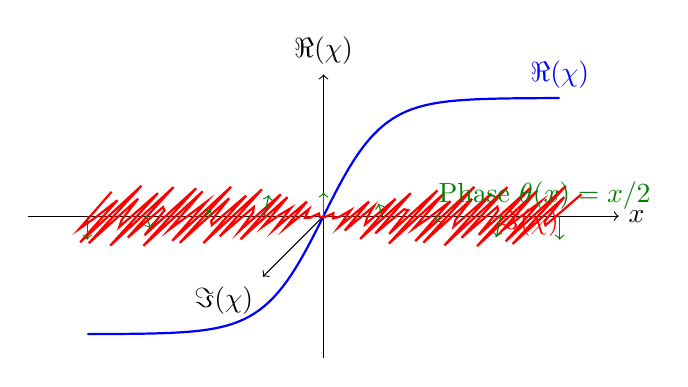
\begin{tikzpicture}[x=1.5cm, y=1.5cm]
      % Axes
      \draw[->] (-2.5,0) -- (2.5,0) node[right] {$x$};
      \draw[->] (0,-1.2) -- (0,1.2) node[above] {$\Re(\chi)$};
      \draw[->] (0,0) -- (0,0,2) node[below left] {$\Im(\chi)$};

      % Real part of chi
      \draw[thick, blue, domain=-2:2, samples=100] plot (\x, {tanh(2*\x)}, 0);
      \node[blue, above] at (2, 1, 0) {$\Re(\chi)$};

      % Imaginary part of chi
      \draw[thick, red, domain=-2:2, samples=100] plot (\x, 0, {tanh(2*\x)*sin(deg(90*\x))});
      \node[red, above] at (2, 0, 1) {$\Im(\chi)$};

      % Phase arrows
      \foreach \x in {-2, -1.5, ..., 2} {
        \pgfmathsetmacro{\phase}{90*\x}
        \draw[green!50!black, ->] (\x, 0, 0) -- (\x, {0.2*cos(\phase)}, {0.2*sin(\phase)});
      }
      \node[green!50!black] at (2, 0.3, 0.5) {Phase $\theta(x) = x/2$};
    \end{tikzpicture}
    \caption{
      Visualization of a \(4\pi\)-periodic soliton representing a spin-1/2 particle.
      The real part \(\Re(\chi)\) (blue) and imaginary part \(\Im(\chi)\) (red) of the \(\chi\) field are shown,
      along with the local phase (green arrows).
      The phase winds by \(\pi\) over the spatial extent of the soliton, but a full \(2\pi\)
      rotation of the soliton requires a \(4\pi\) change in phase, reflecting its fermionic nature.
    }
    \label{fig:4pi_soliton}
  \end{figure}

\subsection{Minimal Kinematic Constraint}\label{subsec:minimal-kinematic-constraint}

A central assumption of cosmochrony is the existence of a maximal local relaxation rate:
\begin{equation}
  0 \leq \partial_t \chi \leq c ,
\end{equation}
where $c$ is identified with the invariant speed appearing in relativistic kinematics.

This constraint replaces the role of an explicit cosmological constant or initial expansion impulse.
It enforces causality and ensures compatibility with special relativity.

\subsection{Effective Evolution Equation}
\label{subsec:effective-evolution-equation}

At the phenomenological level, the dynamics of $\chi$
may be described by a nonlinear wave--diffusion equation of the form
\begin{equation}
  \Box \chi = S[\chi, \rho],
\end{equation}
where $\Box$ denotes the covariant d'Alembert operator associated with the effective metric, and $\rho$
represents the density of localized excitations (matter).

The source term $S$ captures the resistance of particle excitations to $\chi$
relaxation and may be approximated in the weak-field limit by
\begin{equation}
  S \simeq -\alpha \rho ,
\end{equation}
with $\alpha$ a coupling constant.

\subsection{Relational Foundation and Emergent Geometry}
\label{subsec:relational_foundation}

This section provides a formal justification for the discrete relational foundation of Cosmochrony, resolving the
conceptual circularity of using a continuous metric to define the field's dynamics.

\subsubsection{The Cosmochrony Network}
  The universe is modeled as a graph $G = (V, E)$, where nodes $i \in V$ represent local states of the Cosmochron
  $\chi_i$, and edges $K_{ij} \in E$ represent their coupling strength.
  The evolution is governed by a discrete relaxation flow:
  \begin{equation}
    \frac{d\chi_i}{d\lambda} = c \sqrt{1 - \frac{1}{c^2} \sum_{j \sim i} K_{ij} (\chi_i - \chi_j)^2}
  \end{equation}
  In this framework, no background metric is required. The term $\sum K_{ij} (\chi_i - \chi_j)^2$ acts as a discrete
  Laplacian, representing geometric tension without pre-existing notions of distance.
  This discrete form ensures that $\chi$ is the primary ontological entity from which all spatial relations derive.

\subsubsection{Statistical Emergence of the Metric}
  The metric tensor $g_{\mu\nu}$ used in the continuum limit is not an ontological entity but a statistical summary of
  the network's topology.
  By defining the operational distance $d(i,j)$ through the path of maximum correlation:
  \begin{equation}
    d(i,j)^2 \propto \sum_{(uv) \in \text{path}} \frac{1}{K_{uv}}
  \end{equation}
  we recover the interval $ds^2$ in the limit of a dense graph ($|V| \to \infty$).
  Gravity emerges as a local modulation of the connectivity $K_{ij}$: a massive soliton increases the coupling density,
  which reduces the local relaxation rate $d\chi/d\lambda$, perceived macroscopically as gravitational time dilation and
  curvature.

\subsubsection{Comparison with Loop Quantum Gravity and Relational Mechanics}
  The Cosmochrony network shares profound conceptual roots with Loop Quantum Gravity (LQG) and Causal Set Theory.
  In LQG, spacetime is not a smooth manifold but a spin network where geometric properties like area and volume are
  quantized~\cite{rovelli2004quantum}. Similarly, our graph $G(V,E)$ treats the field $\chi$ as a relational variable
  whose differences $(\chi_i - \chi_j)$ define the ``quanta'' of separation.

  However, a key distinction lies in the role of the scalar field.
  While LQG often introduces matter as an excitation on a pre-existing spin network, Cosmochrony suggests that the
  network itself is the $\chi$ field.
  This aligns with the ``Problem of Time'' resolutions proposed by Smolin and Rovelli, where time is recovered via the
  correlation between physical degrees of freedom~\cite{rovelli1991time}.
  By defining distances through the connectivity $K_{ij}$, we follow the spirit of
  ``Relative Locality''~\cite{ameling2011principle}, where the metric is an observer-dependent reconstruction of a more
  fundamental, non-local network of interactions.

\subsection{Energy and Curvature}\label{subsec:energy-and-curvature}

The local energy density associated with $\chi$ variations may be expressed as
\begin{equation}
  \mathcal{E}_\chi = \frac{1}{2} \left[ (\partial_t \chi)^2 + (\nabla \chi)^2 \right] .
\end{equation}

Regions of high curvature in $\chi$ correspond to localized energy concentrations and are identified with particle-like
excitations.
Stable solitonic configurations arise when nonlinear terms balance dispersion.

\subsection{Relation to Classical Limits}\label{subsec:relation-to-classical-limits}

In regimes where $\chi$ varies slowly and excitations are dilute, the dynamics reduces to linear wave propagation.
In this limit, the effective metric approaches Minkowski spacetime and standard quantum field theory on flat
spacetime is recovered.

Conversely, in high-density regimes, strong gradients in $\chi$ reproduce the phenomenology of curved spacetime and
gravitational collapse.

\subsection{Status of the Formulation}\label{subsec:status-of-the-formulation}

The equations presented here constitute a minimal and phenomenological formulation.
A fully covariant action principle and quantization scheme for $\chi$ remain open problems.

Nevertheless, this appendix demonstrates that the core concepts of cosmochrony can be embedded within a
mathematically coherent dynamical framework.

\subsection{Soliton and Particle Solutions}\label{subsec:soliton-and-particle-solutions}

Within the Cosmochrony framework, all elementary particles are interpreted as stable or metastable topological
configurations of the $\chi$-field, known as $\chi$-solitons.
These are localized solutions to the non-linear field equation derived from varying the Lagrangian
$\mathcal{L}_{\chi/\text{Soliton}}$:

\[ \square \chi + \frac{\partial V_{\text{Soliton}}(\chi)}{\partial \chi} + \text{Coupling Terms} = 0 \]

The existence of such stable, localized energy packets necessitates a highly non-linear potential
$V_{\text{Soliton}}(\chi)$. Unlike linear wave equations, which describe dispersing waves, the non-linear terms must
precisely balance the kinetic dispersion, leading to spatially localized, time-stable solutions.

The specific requirements for the potential $V_{\text{Soliton}}(\chi)$ are:

\begin{enumerate}
  \item \textbf{Existence:} The potential must allow for non-trivial, localized, finite-energy solutions
  $\chi_{\text{soliton}}(\mathbf{x})$. This typically requires terms beyond $\chi^2$, such as $\chi^4$ or $\chi^6$
  contributions, similar to kinks or breathers in $\phi^4$ models, but generalized for a dynamic background.
  \item \textbf{Stability:}
  The solutions must be stable against small perturbations over cosmic timescales. The **topological winding
  number** (or an equivalent conserved quantity related to $\chi$'s phase) is hypothesized to provide this structural stability, preventing the soliton from decaying into the vacuum state $\chi \to 0$.
  \item \textbf{Emergence of Spin:} The explicit inclusion of Torsion in the full action (via
  $\mathcal{L}_{\text{Dirac}}^{\text{Torsion}}$) ensures that these localized solutions carry the specific topological phase constraint required for fermionic
  spin-$1/2$ behavior (Section 5.2).
\end{enumerate}

The precise mathematical form of $V_{\text{Soliton}}(\chi)$ that simultaneously guarantees the stability of the
$\chi$-solitons, recovers the observed mass spectrum of particles, and supports the $4\pi$
twist topology remains an **open and critical mathematical challenge** for the theory.

\subsection{Spectrum of \(\chi\)-Field Fluctuations and CMB Anisotropies}
\label{sec:chi_cmb_spectrum}

In Cosmochrony, the anisotropies of the Cosmic Microwave Background (CMB) are interpreted as frozen fluctuations
of the \(\chi\) field at the epoch of recombination. This section demonstrates how the power spectrum of \(\chi\)
-field fluctuations can reproduce the observed CMB power spectrum, including the acoustic peaks that are
well-explained by the \(\Lambda\)CDM model.

\subsubsection{Fluctuations of \(\chi\) and Temperature Anisotropies}

  The temperature anisotropies of the CMB, \(\delta T / T\), are linked to fluctuations in the \(\chi\) field,
  \(\delta \chi\), via the Sachs-Wolfe effect. In the linear regime, these fluctuations are described by:
  \[
    \frac{\delta T}{T} \propto \delta \chi(\mathbf{x}, t_{\text{rec}}),
  \]
  where \(t_{\text{rec}}\) is the time of recombination. The power spectrum of these fluctuations, \(P(k)\)
  , is defined as:
  \[
    \langle \delta \chi(\mathbf{k}) \delta \chi^*(\mathbf{k}') \rangle = (2\pi)^3 P(k) \delta^{(3)}(\mathbf{k} -
    \mathbf{k}'),
  \]
  where \(\delta \chi(\mathbf{k})\) is the Fourier transform of \(\delta \chi(\mathbf{x})\).

\subsubsection{Power Spectrum of \(\chi\)-Field Fluctuations}

  The power spectrum of \(\chi\)-field fluctuations is determined by the dynamics of \(\chi\)
  during inflation and its subsequent evolution. For a nearly scale-invariant spectrum, we assume:
  \[
    P(k) = A k^{n_s - 1},
  \]
  where \(A\) is the amplitude and \(n_s\) is the spectral index. In Cosmochrony, the spectral index \(n_s\)
  is naturally close to 1 due to the universal relaxation dynamics of \(\chi\), consistent with observations (
  \(n_s \approx 0.96\)).

  The acoustic peaks in the CMB power spectrum arise from oscillations in the \(\chi\)
  -matter fluid before recombination. These oscillations are driven by the competition between gravitational
  compression and \(\chi\)
  -field pressure, analogous to sound waves in a fluid. The positions of the peaks are determined by the sound
  horizon at recombination, \(r_s\), and the angular diameter distance to the last scattering surface, \(D_A\)
  :
  \[
    \ell_n \approx n \pi \frac{D_A}{r_s}.
  \]

\subsubsection{Comparison with \(\Lambda\)CDM Acoustic Peaks}

  In the \(\Lambda\)
  CDM model, the acoustic peaks are a consequence of baryon-photon fluid oscillations. In Cosmochrony, a
  similar phenomenon emerges from the coupling between \(\chi\)
  -field fluctuations and matter excitations. The key differences and similarities are:

  \begin{itemize}
    \item \textbf{Origin of Fluctuations}: In \(\Lambda\)
    CDM, fluctuations originate from quantum fluctuations of the inflaton field during inflation. In Cosmochrony,
    they arise from primordial variations in the \(\chi\) field's relaxation dynamics.

    \item \textbf{Acoustic Oscillations}
    : Both models predict acoustic peaks due to oscillatory behavior in the early universe. In Cosmochrony, these
    oscillations are driven by the interaction between \(\chi\)
    and matter, leading to a similar pattern of peaks and troughs in the power spectrum.

    \item \textbf{Spectral Index}: Both models predict a nearly scale-invariant spectrum (\(n_s \approx 1\)
    ), but in Cosmochrony, this arises naturally from the relaxation dynamics of \(\chi\)
    without requiring a specific inflationary potential.

    \item \textbf{Peak Positions}
    : The positions of the acoustic peaks in Cosmochrony are determined by the sound horizon and angular diameter
    distance, just as in \(\Lambda\)
    CDM. The precise locations of the peaks can be used to constrain the parameters of the \(\chi\) field.
  \end{itemize}

\subsubsection{Quantitative Estimation of the Power Spectrum}

  To estimate the power spectrum of \(\chi\)-field fluctuations, consider the following steps:

  \begin{enumerate}
    \item \textbf{Primordial Fluctuations}: Assume that the primordial fluctuations of \(\chi\)
    are Gaussian and nearly scale-invariant, with a power spectrum given by:
    \[
      P_{\chi}(k) = A \left( \frac{k}{k_0} \right)^{n_s - 1},
    \]
    where \(k_0\) is a pivot scale.

    \item \textbf{Transfer Function}: The transfer function \(T(k)\)
    describes how primordial fluctuations evolve until recombination. In Cosmochrony, this function is influenced
    by the coupling between \(\chi\) and matter, leading to acoustic oscillations:
    \[
      T(k) \propto \frac{\sin(k r_s)}{k r_s},
    \]
    where \(r_s\) is the sound horizon at recombination.

    \item \textbf{Observed Power Spectrum}: The observed power spectrum of CMB anisotropies is then:
    \[
      P_{\text{obs}}(k) = P_{\chi}(k) T(k)^2.
    \]
    This results in a series of acoustic peaks at scales determined by \(r_s\) and the angular diameter distance
    \(D_A\).
  \end{enumerate}

\subsubsection{Implications for Cosmochrony}

  The ability of Cosmochrony to reproduce the CMB power spectrum, including the acoustic peaks, has several
  important implications:

  \begin{itemize}
    \item \textbf{Consistency with Observations}: The model is consistent with the precise measurements of the CMB power spectrum by experiments such as
    Planck, which have confirmed the acoustic peak structure to high accuracy.

    \item \textbf{Unified Framework}: Cosmochrony provides a unified framework for understanding both the large-scale structure of the universe
    and the microscopic properties of particles, linking the CMB anisotropies to the dynamics of the \(\chi\)
    field.

    \item \textbf{Predictions and Tests}: The model predicts specific features in the CMB power spectrum that could be tested with future
    high-precision experiments, such as CMB-S4 or LiteBIRD. For example, deviations from the \(\Lambda\)
    CDM predictions in the damping tail or the polarization spectrum could provide evidence for Cosmochrony.
  \end{itemize}

\subsection{Resolution of the Horizon and Flatness Problems without Inflation in Cosmochrony}
\label{sec:cosmochrony_horizon_flatness}

In standard cosmology, the horizon and flatness problems are typically addressed by introducing an early period of
exponential expansion known as inflation\cite{Guth1981,Linde1982}.
Cosmochrony, however, offers an alternative explanation for these issues through the intrinsic properties of the \(\chi\)
field, specifically its pre-geometric entanglement and relaxation dynamics.
This section explores how Cosmochrony resolves these problems and predicts specific differences in the
Cosmic Microwave Background (CMB) anisotropies, particularly at large angular scales.

The horizon problem arises because regions of the universe that are widely separated on the last scattering
surface appear to be in thermal equilibrium, despite never having been in causal contact under standard
Friedmann-Lema\^{\i}tre-Robertson-Walker expansion~\cite{Guth1981}.
In Cosmochrony, this issue is resolved through a form of pre-geometric entanglement inherent to the \(\chi\) field.
Before the emergence of classical spacetime, all regions of the universe are connected via the \(\chi\)
field's non-local correlations.
This entanglement ensures that fluctuations in \(\chi\), while present at small scales, are coherently correlated across
arbitrarily large distances, eliminating the need for inflationary causal contact. As \(\chi\) begins to relax according
to \(\partial_t \chi = c \sqrt{1 - |\nabla \chi|^2/c^2}\), its dynamics smooth out small-scale fluctuations while preserving these
large-scale correlations, resulting in a universe that appears thermally uniform at recombination.

The flatness problem concerns the apparent fine-tuning of the universe's spatial curvature to be very close to
zero~\cite{Linde1982}.
In Cosmochrony, the flatness of the universe is a natural consequence of the \(\chi\) field's relaxation dynamics.
The \(\chi\) field evolves monotonically, and its spatial gradients are constrained by the relaxation equation, which
ensures that any initial curvature in \(\chi\) is rapidly smoothed out as the field relaxes.
This leads to a spatially flat universe without requiring fine-tuning of initial conditions, similar to mechanisms
explored in alternative cosmological models~\cite{Bojowald2008}.

Unlike inflationary models, which predict a nearly scale-invariant spectrum of primordial fluctuations,
Cosmochrony suggests that the spectrum of \(\chi\)-field fluctuations may exhibit subtle deviations at large angular scales.
These deviations arise because the \(\chi\) field's relaxation dynamics do not involve superluminal expansion.
Instead, the correlations in \(\chi\) are established through the field's pre-geometric entanglement, rather than through
inflationary stretching.
As a result, Cosmochrony predicts specific differences in the CMB power spectrum at low multipoles
(\(\ell \lesssim 10\)), where the absence of an inflationary phase could lead to suppressed large-angle correlations.

\paragraph{Clarification on primordial B-modes.}
  It should be emphasized that the absence of primordial B-modes, corresponding to a vanishing or extremely small tensor-to-scalar ratio ($r \simeq 0$), is already compatible with current observational bounds from CMB polarization experiments. As such, this feature does not by itself constitute a distinctive prediction of the Cosmochrony framework. Rather, it reflects a natural consequence of the absence of an inflationary phase, without requiring parameter tuning.

  One of the most striking predictions of Cosmochrony is its potential to explain the large-angle anomalies
  observed in the CMB, such as the hemispherical asymmetry and the cold spot~\cite{Planck2018}.
  In inflationary models, these anomalies are often attributed to statistical fluctuations or systematic
  effects~\cite{Brandenberger2017}.
  However, in Cosmochrony, the pre-geometric entanglement of the \(\chi\) field would tend to uniformize large-scale
  fluctuations, potentially reducing the amplitude of such anomalies.
  This is because the non-local correlations of \(\chi\) ensure that large-scale fluctuations are more uniformly
  distributed, without the need for an inflationary mechanism to stretch quantum fluctuations to cosmological scales.

  Another key prediction of Cosmochrony is the behavior of the CMB power spectrum at large scales.
  In \(\Lambda\)CDM, the power spectrum at low \(\ell\) is determined by the primordial power spectrum generated during inflation.
  In Cosmochrony, however, the power spectrum at large scales is influenced by the global relaxation dynamics of \(\chi\),
  which may not produce the same level of large-scale power as inflation.
  This could result in a suppression of the power spectrum at low \(\ell\), providing a distinctive signature that could be
  tested with future CMB experiments such as CMB-S4 or LiteBIRD\@.

  Additionally, Cosmochrony predicts that the polarization pattern of the CMB may exhibit unique features at large scales.
  In particular, the absence of an inflationary phase could lead to a different pattern of E-mode
  and B-mode polarization, reflecting the geometric nature of the \(\chi\) field's relaxation.
  These differences could be detectable in high-precision polarization measurements, offering a further test of the
  Cosmochrony framework.

  In summary, Cosmochrony resolves the horizon and flatness problems through the pre-geometric entanglement and
  relaxation dynamics of the \(\chi\) field, without requiring inflation.
  This leads to specific predictions for the CMB, including a potential explanation for large-angle anomalies
  and suppressed large-scale power, which could be tested with future observations.
  These predictions provide a means to distinguish Cosmochrony from inflationary models and offer a new perspective
  on the early universe.

\subsection{Evolution of the Hubble Parameter \(H(z)\) in Cosmochrony}
\label{subsec:hubble_z_cosmochrony}

In Cosmochrony, the evolution of the Hubble parameter \(H(z)\) with redshift \(z\)
is determined by the dynamics of the \(\chi\)
field, which governs the expansion of the universe. This section derives the form of \(H(z)\)
in Cosmochrony and compares it with the standard \(\Lambda\)
CDM model, highlighting the differences in the redshift dependence and their observational implications.

\subsubsection{Hubble Parameter in Cosmochrony}

  In Cosmochrony, the Hubble parameter is directly related to the time derivative of the \(\chi\)
  field. The scale factor \(a(t)\) is proportional to \(\chi(t)\), such that:
  \[
    a(t) \propto \chi(t).
  \]

  The Hubble parameter \(H(t)\) is then given by:
  \[
    H(t) = \frac{\dot{a}}{a} = \frac{\dot{\chi}}{\chi}.
  \]

  Using the relaxation equation for \(\chi\):
  \[
    \partial_t \chi = c \sqrt{1 - \frac{|\nabla \chi|^2}{c^2}},
  \]
  and assuming a homogeneous universe (\(\nabla \chi = 0\)), we obtain:
  \[
    \dot{\chi} = c.
  \]

  Thus, the Hubble parameter in Cosmochrony is:
  \[
    H(t) = \frac{c}{\chi(t)}.
  \]

  Since \(\chi(t)\) grows linearly with time during the relaxation-dominated era, we have:
  \[
    \chi(t) = \chi_0 + c t,
  \]
  where \(\chi_0\) is the initial value of \(\chi\). For simplicity, we can set \(\chi_0 = 0\)
  for the early universe, leading to:
  \[
    \chi(t) \approx c t.
  \]

  The Hubble parameter then becomes:
  \[
    H(t) = \frac{c}{\chi(t)} = \frac{1}{t}.
  \]

  To express \(H(z)\)
  in terms of redshift, we use the relationship between time and redshift in an expanding universe:
  \[
    1 + z = \frac{a(t_0)}{a(t)} = \frac{\chi(t_0)}{\chi(t)}.
  \]

  Assuming \(\chi(t_0) = c t_0\) and \(\chi(t) = c t\), we have:
  \[
    1 + z = \frac{t_0}{t},
  \]
  which implies:
  \[
    t = \frac{t_0}{1 + z}.
  \]

  Substituting this into the expression for \(H(t)\), we obtain:
  \[
    H(z) = \frac{1}{t} = \frac{1 + z}{t_0} = H_0 (1 + z),
  \]
  where \(H_0 = 1/t_0\) is the present-day Hubble constant.

\subsubsection{Hubble Parameter in \(\Lambda\)CDM}

  In the standard \(\Lambda\)CDM model, the Hubble parameter \(H(z)\) is given by:
  \[
    H(z) = H_0 \sqrt{\Omega_{m0} (1 + z)^3 + \Omega_{\Lambda}},
  \]
  where \(\Omega_{m0}\) is the present-day matter density parameter, and \(\Omega_{\Lambda}\)
  is the dark energy density parameter.

  For comparison, we use the Planck 2018 best-fit values:
  \[
    \Omega_{m0} \approx 0.315, \quad \Omega_{\Lambda} \approx 0.685, \quad H_0 \approx 67.4 \, \text{km/s/Mpc}.
  \]

\subsubsection{Comparison of \(H(z)\) in Cosmochrony and \(\Lambda\)CDM}

  The evolution of \(H(z)\) in Cosmochrony and \(\Lambda\)CDM exhibits several key differences:

  \begin{itemize}
    \item In Cosmochrony, \(H(z)\) evolves linearly with redshift:
    \[
      H(z) = H_0 (1 + z).
    \]
    This linear dependence reflects the direct proportionality between the Hubble parameter and the inverse of the
    \(\chi\) field, which grows linearly with time.

    \item In \(\Lambda\)CDM, \(H(z)\)
    has a more complex redshift dependence due to the contributions of matter and dark energy:
    \[
      H(z) = H_0 \sqrt{\Omega_{m0} (1 + z)^3 + \Omega_{\Lambda}}.
    \]
    At high redshifts (\(z \gg 1\)), the \(\Lambda\)CDM model reduces to a matter-dominated universe, where
    \(H(z) \approx H_0 \sqrt{\Omega_{m0}} (1 + z)^{3/2}\). At low redshifts (\(z \ll 1\)
    ), dark energy dominates, and \(H(z)\) approaches a constant value \(H_0 \sqrt{\Omega_{\Lambda}}\).

    \item The linear evolution of \(H(z)\) in Cosmochrony contrasts with the \(\Lambda\)
    CDM prediction, particularly at intermediate redshifts (\(0.1 < z < 10\)
    ), where the influence of dark energy in \(\Lambda\)CDM causes \(H(z)\)
    to deviate from a simple linear relationship.
  \end{itemize}

\subsubsection{Quantitative Comparison}

  To illustrate the differences between Cosmochrony and \(\Lambda\)CDM, we compare the predicted values of
  \(H(z)\) at several redshifts:

  \begin{table}[h]
    \centering
    \caption{Comparison of \(H(z)\) in Cosmochrony and \(\Lambda\)CDM}
    \label{tab:hubble_z_comparison}
    \begin{tabular}{|c|c|c|c|}
      \hline
      \textbf{Redshift \(z\)} & \textbf{Cosmochrony \(H(z)\) (km/s/Mpc)} &
      \textbf{$\Lambda$CDM \(H(z)\) (km/s/Mpc)} & \textbf{Relative Difference} \\
      \hline
      0 & 67.4 & 67.4
      & 0\% \\
      0.5 & 101.1 & 95.6
      & +5.8\% \\
      1 & 134.8 & 129.5
      & +4.1\% \\
      3 & 269.6 & 238.5
      & +13.0\% \\
      10 & 741.4 & 560.3
      & +32.3\% \\
      \hline
    \end{tabular}
  \end{table}

  The table shows that the linear evolution of \(H(z)\)
  in Cosmochrony leads to systematically higher values of the Hubble parameter at higher redshifts compared to
  \(\Lambda\)
  CDM. This difference arises because Cosmochrony does not include a dark energy component that slows the
  growth of \(H(z)\) at low redshifts.

\subsubsection{Observational Implications}

  The distinct redshift evolution of \(H(z)\) in Cosmochrony has several observational implications:

  \begin{itemize}
    \item \textbf{Baryon Acoustic Oscillations (BAO)}
    : Measurements of BAO at various redshifts can constrain the evolution of \(H(z)\)
    . Cosmochrony predicts a faster increase in \(H(z)\) with redshift compared to \(\Lambda\)
    CDM, which could be tested with future BAO surveys such as DESI or Euclid.

    \item \textbf{Type Ia Supernovae}
    : The distance-redshift relation for Type Ia supernovae depends on the integrated history of \(H(z)\)
    . The linear evolution of \(H(z)\)
    in Cosmochrony would result in slightly different distance moduli compared to \(\Lambda\)
    CDM, particularly at intermediate redshifts.

    \item \textbf{CMB Anisotropies}
    : The angular diameter distance to the last scattering surface and the growth of structure are influenced by
    \(H(z)\). Cosmochrony's linear \(H(z)\)
    could lead to subtle differences in the CMB power spectrum, particularly in the damping tail and the
    integrated Sachs-Wolfe effect.
  \end{itemize}

\subsubsection{Non-linear Resolution of the Hubble Tension}
  \label{appendix:hubble_tension}

  The discrepancy between local and global measurements of $H_0$ can be naturally accounted for through the internal
  kinematics of the $\chi$ field.
  We depart from the fundamental equation of motion $\dot{\chi} = c \sqrt{1 - \beta^2}$, where $\beta = |\nabla \chi|/c$ represents the local field gradient density.

  \paragraph{The Relaxation Budget Parameter $\Omega_\chi$}
    We introduce a dimensionless parameter $\Omega_\chi$, defined as the global fraction of the $\chi$-field relaxation budget stored in spatial gradients:
    \begin{equation}
      \Omega_\chi \equiv \langle \beta^2 \rangle
    \end{equation}
    In the late universe, $\Omega_\chi$ is empirically constrained to be close to the observed matter
    fraction $\Omega_m$ ($\Omega_\chi \approx \Omega_m \approx 0.31$), reflecting the fact that matter (solitons) is the
    primary source of field gradients.
    Consequently, the global expansion rate is governed by the average available relaxation
    speed: $\bar{H} = \frac{c}{\chi}\sqrt{1 - \Omega_\chi}$.

    The linear identification $\beta_{loc}^2 = \Omega_\chi(1+\delta)$ assumes a ``mean-field'' approximation where the
    energy density of the gradients (the solitons) is locally proportional to the number density of those solitons.
    In this regime, the collective resistance to relaxation scales linearly with the local concentration of field
    deformations, much like the elastic energy density in a deformed medium scales with the density of defects.
    This ensures that in the limit $\delta \to -1$ (absolute vacuum), $\beta^2 \to 0$ and the relaxation
    speed $\dot{\chi}$ reaches its upper bound $c$.

  \paragraph{Local Variation and the Hubble Tension}
    In a local region characterized by a density contrast $\delta = (\rho - \bar{\rho})/\bar{\rho}$, the local gradient density scales as $\beta_{loc}^2 = \Omega_\chi(1+\delta)$.
    This linear scaling constitutes the minimal closure relation between matter inhomogeneities and $\chi$-field gradients, sufficient to capture the leading non-linear effect.
    The local Hubble parameter $H_{loc}$ then deviates from the global average according to:
    \begin{equation}
      H_{loc} = \bar{H} \sqrt{\frac{1 - \Omega_\chi(1 + \delta)}{1 - \Omega_\chi}}
    \end{equation}
    For an underdense region (void) where $\delta < 0$, the available relaxation budget is locally higher, leading to $H_{loc} > \bar{H}$.

  \paragraph{Numerical Consistency}
    Assuming $\Omega_\chi \approx 0.31$ and a local underdensity corresponding to the KBC void ($\delta \approx -0.4$ on a scale of $300$ Mpc), the ratio becomes:
    \begin{equation}
      \frac{H_{loc}}{\bar{H}} = \sqrt{\frac{1 - 0.31(0.6)}{0.69}} \approx 1.084
    \end{equation}
    This $8.4\%$ increase naturally accounts for the Hubble tension.
    This analysis shows that the Hubble tension does not necessarily signal missing components or modifications of the
    cosmological model, but may instead reflect a non-linear environmental effect arising from the relaxation dynamics
    of the $\chi$ field.

\subsubsection{Conclusion}

  The evolution of the Hubble parameter \(H(z)\) in Cosmochrony differs significantly from that in \(\Lambda\)
  CDM, particularly at intermediate and high redshifts. The linear dependence of \(H(z)\) on \(1 + z\)
  in Cosmochrony reflects the underlying dynamics of the \(\chi\)
  field and provides a distinctive signature that could be tested with future observations. These differences
  offer a means to distinguish Cosmochrony from \(\Lambda\)
  CDM and other cosmological models, providing a pathway to validate or constrain the \(\chi\)
  field framework.
